% This is "sig-alternate.tex" V2.1 April 2013
% This file should be compiled with V2.5 of "sig-alternate.cls" May 2012
%
% This example file demonstrates the use of the 'sig-alternate.cls'
% V2.5 LaTeX2e document class file. It is for those submitting
% articles to ACM Conference Proceedings WHO DO NOT WISH TO
% STRICTLY ADHERE TO THE SIGS (PUBS-BOARD-ENDORSED) STYLE.
% The 'sig-alternate.cls' file will produce a similar-looking,
% albeit, 'tighter' paper resulting in, invariably, fewer pages.
%
% ----------------------------------------------------------------------------------------------------------------
% This .tex file (and associated .cls V2.5) produces:
%       1) The Permission Statement
%       2) The Conference (location) Info information
%       3) The Copyright Line with ACM data
%       4) NO page numbers
%
% as against the acm_proc_article-sp.cls file which
% DOES NOT produce 1) thru' 3) above.
%
% Using 'sig-alternate.cls' you have control, however, from within
% the source .tex file, over both the CopyrightYear
% (defaulted to 200X) and the ACM Copyright Data
% (defaulted to X-XXXXX-XX-X/XX/XX).
% e.g.
% \CopyrightYear{2007} will cause 2007 to appear in the copyright line.
% \crdata{0-12345-67-8/90/12} will cause 0-12345-67-8/90/12 to appear in the copyright line.
%
% ---------------------------------------------------------------------------------------------------------------
% This .tex source is an example which *does* use
% the .bib file (from which the .bbl file % is produced).
% REMEMBER HOWEVER: After having produced the .bbl file,
% and prior to final submission, you *NEED* to 'insert'
% your .bbl file into your source .tex file so as to provide
% ONE 'self-contained' source file.
%
% ================= IF YOU HAVE QUESTIONS =======================
% Questions regarding the SIGS styles, SIGS policies and
% procedures, Conferences etc. should be sent to
% Adrienne Griscti (griscti@acm.org)
%
% Technical questions _only_ to
% Gerald Murray (murray@hq.acm.org)
% ===============================================================
%
% For tracking purposes - this is V2.0 - May 2012

\documentclass{sig-alternate-05-2015}
\usepackage{times}
\usepackage{helvet}
\usepackage{courier}
\usepackage{graphicx}
\usepackage{booktabs} % for pretty table rules
\usepackage{hyperref}
\usepackage[T1]{fontenc}

\setlength{\pdfpagewidth}{8.5in}
\setlength{\pdfpageheight}{11in}
\pdfinfo{
/Title Monitoring the Gender Gap with Wikidata Human Gender Indicators
/Author BLINDED}

\begin{document}

% Copyright
\setcopyright{acmcopyright}
%\setcopyright{acmlicensed}
%\setcopyright{rightsretained}
%\setcopyright{usgov}
%\setcopyright{usgovmixed}
%\setcopyright{cagov}
%\setcopyright{cagovmixed}


% DOI
\doi{10.475/123_4}

% ISBN
\isbn{123-4567-24-567/08/06}

%Conference
\conferenceinfo{PLDI '13}{June 16--19, 2013, Seattle, WA, USA}

\acmPrice{\$15.00}

%
% --- Author Metadata here ---
\conferenceinfo{WOODSTOCK}{'97 El Paso, Texas USA}
%\CopyrightYear{2007} % Allows default copyright year (20XX) to be over-ridden - IF NEED BE.
%\crdata{0-12345-67-8/90/01}  % Allows default copyright data (0-89791-88-6/97/05) to be over-ridden - IF NEED BE.
% --- End of Author Metadata ---

\title{Monitoring the Gender Gap with Wikidata Human Gender Indicators}

%
% You need the command \numberofauthors to handle the 'placement
% and alignment' of the authors beneath the title.
%
% For aesthetic reasons, we recommend 'three authors at a time'
% i.e. three 'name/affiliation blocks' be placed beneath the title.
%
% NOTE: You are NOT restricted in how many 'rows' of
% "name/affiliations" may appear. We just ask that you restrict
% the number of 'columns' to three.
%
% Because of the available 'opening page real-estate'
% we ask you to refrain from putting more than six authors
% (two rows with three columns) beneath the article title.
% More than six makes the first-page appear very cluttered indeed.
%
% Use the \alignauthor commands to handle the names
% and affiliations for an 'aesthetic maximum' of six authors.
% Add names, affiliations, addresses for
% the seventh etc. author(s) as the argument for the
% \additionalauthors command.
% These 'additional authors' will be output/set for you
% without further effort on your part as the last section in
% the body of your article BEFORE References or any Appendices.

\numberofauthors{5} %  in this sample file, there are a *total*
% of EIGHT authors. SIX appear on the 'first-page' (for formatting
% reasons) and the remaining two appear in the \additionalauthors section.
%
\author{
% You can go ahead and credit any number of authors here,
% e.g. one 'row of three' or two rows (consisting of one row of three
% and a second row of one, two or three).
%
% The command \alignauthor (no curly braces needed) should
% precede each author name, affiliation/snail-mail address and
% e-mail address. Additionally, tag each line of
% affiliation/address with \affaddr, and tag the
% e-mail address with \email.
%
% 1st. author
\alignauthor
Author Blinded\\
       \affaddr{blind}\\
       \affaddr{blind}\\
       \affaddr{blind}\\
       \email{blind}
% 2nd. author
\alignauthor
Author Blinded\\
       \affaddr{blind}\\
       \affaddr{blind}\\
       \affaddr{blind}\\
       \email{blind}
% 3rd. author
\alignauthor 
Author Blinded\\
       \affaddr{blind}\\
       \affaddr{blind}\\
       \affaddr{blind}\\
       \email{blind}
\and  % use '\and' if you need 'another row' of author names
% 4th. author
\alignauthor 
Author Blinded\\
       \affaddr{blind}\\
       \affaddr{blind}\\
       \affaddr{blind}\\
       \email{blind}
% 5th. author
\alignauthor 
Author Blinded\\
       \affaddr{blind}\\
       \affaddr{blind}\\
       \affaddr{blind}\\
       \email{blind}
}
% There's nothing stopping you putting the seventh, eighth, etc.
% author on the opening page (as the 'third row') but we ask,
% for aesthetic reasons that you place these 'additional authors'
% in the \additional authors block, viz.
% Just remember to make sure that the TOTAL number of authors
% is the number that will appear on the first page PLUS the
% number that will appear in the \additionalauthors section.

\maketitle
\begin{abstract}
The gender gap in Wikipedia's content, specifically in the representation of women in biographies is well-known, but has been difficult to measure. Furthermore the impacts of efforts to address this gender gap have received little attention. To investigate we utilise Wikidata, the database that feeds Wikipedia, and introduce the ``Wikidata Human Gender Indicators'' (WHGI), an open source, longitudinal, biographical dataset that can provide insights into gender disparities across time, space, culture, occupation and language. Through these lenses we show how women's representation is changing along 11 dimensions. Validations of WHGI are presented against three exogenous datasets: the world's historical population, ``traditional'' gender-disparity indices (GDI, GEI, GGGI and SIGI), and occupational gender according to the US Bureau of Labor Statistics. Furthermore, to demonstrate its general use in research, we revisit previous published findings on Wikipedia's gender bias that can be strengthened by WHGI. 
\end{abstract}


%
% The code below should be generated by the tool at
% http://dl.acm.org/ccs.cfm
% Please copy and paste the code instead of the example below. 
%
\begin{CCSXML}
<ccs2012>
 <concept>
  <concept_id>10010520.10010553.10010562</concept_id>
  <concept_desc>Example</concept_desc>
  <concept_significance>500</concept_significance>
 </concept>

\end{CCSXML}

\ccsdesc[500]{Example~Example}


%
% End generated code
%

%
%  Use this command to print the description
%
\printccsdesc

% We no longer use \terms command
%\terms{Theory}

\keywords{Gender Disparities, Wikipedia, Wikidata, Biographical Database}

\section{Introduction}

Gender inequality is a long-standing social problem which affects many aspects of society. Worldwide, cultural ideologies have created scenarios which make women more prone to health issues \cite{world_health_organization_women_2009}. Likewise in education, attitudes create a systemic gender bias in opportunity \cite{heward_gender_1999}. And, famously, incomes for identical jobs are lower for women \cite{burstein_equal_????}.

Statistical gender indicators are critically important to understanding gender inequality \cite{klasen_gender-related_2004}. Many indicators (single measures) and indices (compound measures) have been proposed, such as The Gender Development Index from the United Nations Development and the Global Gender Gap Index from the World Economic Forum. Still there are some features lacking among the current gender indicators. First, the most frequent ones are released annually, which does not allow for fine-grained analysis. Also they measure only recent history, which limits analysis of the past. And lastly they are not open source, which means verification and remixing is more difficult.


At the same time Wikipedia's \textit{editor} gender gap has come to light as deeply gender-disparate, and received media attention for it \cite{cohen_wikipedia_2011}. Responses, however, are not focused solely on editors, but also \textit{biographical} coverage. Gender-focused Wikipedia editing communities create and improve biographies to combat systemic bias, but their large scale effect is unknown. Luckily, new capabilities to record gender via Wikidata, the database that feeds Wikipedia, make encyclopedia-scale descriptions of gender increasingly tractable and accurate.

We introduce a weekly-updated, all-recorded-history level, open source dataset that can provide insights into gender disparities across time, space, culture, occupation and language. ``Wikidata Human Gender Indicators'' (WHGI) is a dataset consisting  of 11 separate indicators on the gender representation of humans in Wikidata. WHGI is open data and available for download at \url{WEBSITE BLINDED}, where we also display visualizations. 

Considering the work in indicator research, the Wikipedia Gender Gap, and the introduction of Wikidata, we ask the following research questions:
\begin{itemize}
\item\textbf{RQ1a} Can we create gender disparity indicators based on the humans in Wikidata?
\item\textbf{RQ1b} To what extent do these indicators reflect real world gender disparities?
\item\textbf{RQ2} How can the Wikipedia community use gender disparity indicators?
\item\textbf{RQ3} How could existing research benefit from gender disparity indicators?
\end{itemize}

The rest of this paper is organized around the four research questions: we begin by describing the format of Wikidata and statistics of humans contained in it. We propose WHGI - a gender disparity indicator. Then, we present 3 validation measures utilizing ground truths from the US Census Bureau, Bureau for Labor Statistics, and United Nations Development Program. This check shows that WHGI is aligned with other indicators in use, confirming its potential for general utility. Third, we illustrate how Wikipedia editing communities could use our dataset to chart their progress, and help their cause under the philosophy of ``what gets measured, gets fixed.'' Finally, we show how WHGI can be used by researchers to better understand gender disparity phenomenon and other content improvement movements, in ways traditional indicators can't.


\section{Related Work}

The thread of research on Wikipedia's gender biases has grown since the finding that Wikipedia's editors are largely not women \cite{glott2010wikipedia} \cite{lam_wp:clubhouse?:_2011}, ranging from 13\% to 16\% \cite{hill_wikipedia_2013}. This imbalance has been attributed to an internet skills gap \cite{hargittai_mind_2015} and the editing community's internal culture \cite{lam_wp:clubhouse?:_2011}. 

More and more, in addition to investigations of the Wikipedia \textit{editor gender gap} researchers have also been interrogating the character of its \textit{biography gender gap}. Early studies found that Wikipedia excluded notable women more than its counterparts \cite{reagle_gender_2011}. More recently \cite{wagner_its_2015} it was shown that while coverage of women in large Wiki\-pedias is not less than other reference works, the wording with which women are portrayed is different and focuses more on romance and family. Women also tend to be less central in the link graph of Wikipedia \cite{10.1371/journal.pone.0114825}. These linguistic and network findings were confirmed by \cite{graells-garrido_first_2015}, who also showed evidence of stereotyping in metadata. Intersectionally, in terms of socio-economic biases, the level of contributions to a Wikipedia language are associated with the wealth of the country they originate from \cite{rask_reach_2008}.

Yet in popular mind-share there persists a sentiment that denies that any of this is a problem \cite{eckert_retriggering_2013}. Luckily, experiments are showing that awareness of Wikipedia's gender issues is a strategy that can alleviate the problem \cite{hinnosaar_gender_2015}, for which more methods are always needed.

\begin{figure}
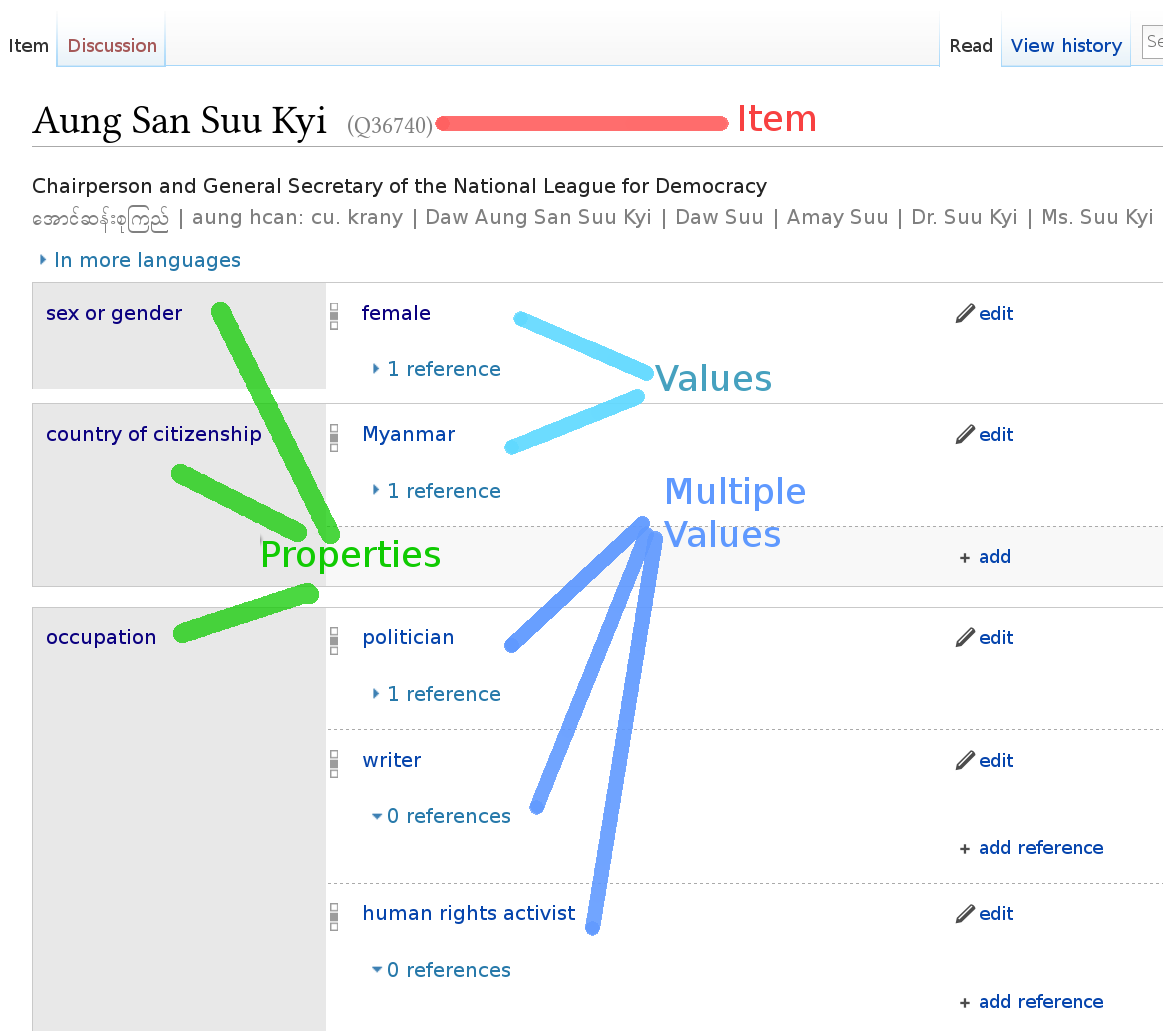
\includegraphics[width=\columnwidth]{figures/aung_explainer_small.png} 
\caption{Example Wikidata Human Item of Aung San Suu Kyi}
\label{fig:aung}
\end{figure}

Wikidata, offers new opportunities to analyze culture programmatically. Launched in 2012, Wikidata is designed to host structured data that is \textit{multilingual} (so there is only one edition) and \textit{plural} (can support many competing facts) \cite{vrandecic_wikidata:_2014}.  These features make Wikidata well-suited for all Wikipedias to collaboratively store facts about the world. If an Italian Wikipedian stores information about the population of ancient Rome, that information is then available to every other Wikipedia with a short code snippet. Every language collaborating together has meant that Wikidata has become a massive free open knowledge-base in its own right, containing over 40 million facts \cite{krotzsch_how_????}.

As a knowledge-base, Wikidata is slowly proving its worth for research. Early on Wikidata showed the importance of multilingual Wikipedians in reducing self-focus bias of language editions. \cite{hale_multilinguals_2014} Wikidata has also been used to find popular connections between nationalities and occupations \cite{goldfarb_quantifying_2015}. Or take the fact that all human and mouse genes have been imported into Wikidata \cite{mitraka_wikidata:_2015}, for an internet-wide community effort to find links between genes, drugs and diseases \cite{burgstaller-muehlbacher_wikidata_2015}. All of these tasks would be difficult to do without Wikidata.


\section{Method}

Wikidata is a general database consisting of \textit{items} which are described by \textit{properties} that take on \textit{values}. Our interest is in biographies of people, that is, any item which has the property \textit{instance of} with value \textit{human} \footnote{As Wikidata is intentionally multilingual, items, properties and values are actually referenced by number. So ``instance of: human'' is ``P31:Q5'' in Wikidata terms }. For each human item we find the corresponding values of \textit{gender}, \textit{date of birth}, \textit{date of death}, \textit{place of birth}, \textit{citizenship}, \textit{ethnic group}, \textit{field of work}, and \textit{occupation} \footnote{These correspond to Wikidata properties P21, P569, P570, P19, P27, P172, P101, and P106 respectively.} In Figure \ref{fig:aung}, we illustrate the semantics of a Wikidata Human on the item for Aung San Suu Kyi.
 
\begin{table}
\caption{An excerpt of the January 3\textsuperscript{rd} 2016 date of birth indicator illustrating the gender aggregation of Wikidata by birth year. The earliest humans in Wikidata are two men born in 4203 b.c.e., births peak in the 1980's (see Figure \ref{fig:genderbydob}), and there are thirteen notable 1-year-olds in Wikidata. Notice the inclusion of non-binary genders as they are recorded in Wikidata, as well as biographies without any gender recorded.}
\begin{tabular} {p{0.75cm}p{0.75cm}p{0.75cm}p{0.75cm}p{0.75cm}p{0.75cm}p{0.75cm}}
\toprule
date of birth & no gender & trans-gender female & gender-queer & ka-thoey & female & male \\
\midrule
4203 \small{(B.C.E.)} & & & & & & 2   \\ 
$\cdots$ &  &  &  & &  &    \\ 
1981 & 849 & 1 &  & 1 &5,042 & 14,461 \\ 
1982 & 861 & 2 &  & &5,132 & 14,372  \\ 
1983 & 864 & 3 &  & &5,078 & 14,520  \\ 
1984 & 830 & 3 & 1 & &5,372 & 14,558   \\ 
1985 & 777 & 4 &  & &5,400 & 14,664  \\ 
$\cdots$ &  &  &  & &  &    \\ 
2015 & 6 &  &  & & 4 & 3  \\ 
\bottomrule
\end{tabular}
\label{table:dob}
\end{table}

For each of the above eight properties we create an ``indicator'' by aggregating the dataset on that property, but disaggregating on gender. Take for example the date of birth indicator, it has one row per year found as a date of birth, and one column per gender represented in Wikidata. See a sample excerpt of the date of birth indicator in Table \ref{table:dob}, and it's visualization in Figure \ref{fig:genderbydob}. Notice in particular that not every human with a date of birth has a gender (recorded as \textit{no gender} in our data), and that Wikidata's community has a non-binary view of gender and includes humans which are neither \textit{male} nor \textit{female}. In addition to the eight indicators made directly from properties, we include three more which feature augmented data. The ``language'' indicator is based on the Wikipedia languages in which a human is represented (shown in Figure \ref{fig:genderbylang}). Finally we include geographic aggregations of citizenship, place of birth and ethnic group into indicators called \textit{culture}\footnote{based on the Inglehart-Welzel cultural map of the world}, and \textit{worldmap} (shown in Figure \ref{fig:genderbycountry}).


\begin{figure}
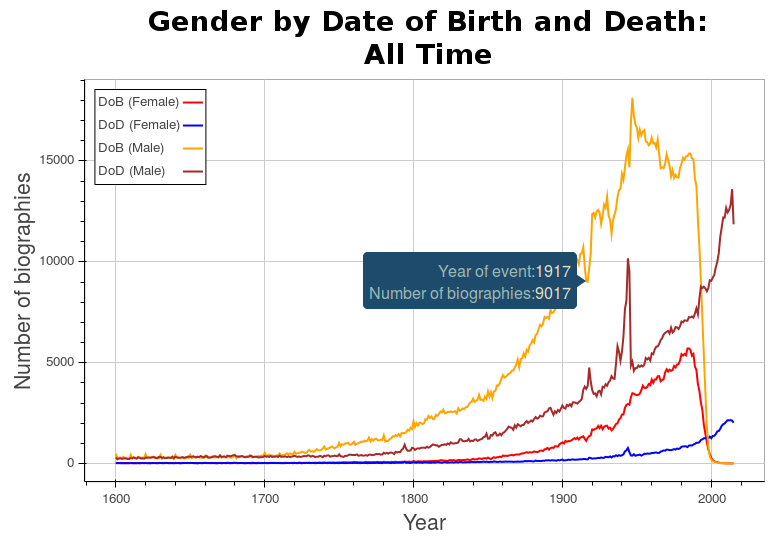
\includegraphics[width=\columnwidth]{figures/genderbydob.png} 
\caption{The total of Wikidata gendered biographies aggregated by date of birth and date of death. This data is represents the January 3\textsuperscript{rd} 2016 snapshot. See the noticeable spikes in death for men around World War II. Births drop about 20 years before the current year, as younger people tend not to be notable.}
\label{fig:genderbydob}
\end{figure}

\begin{figure}
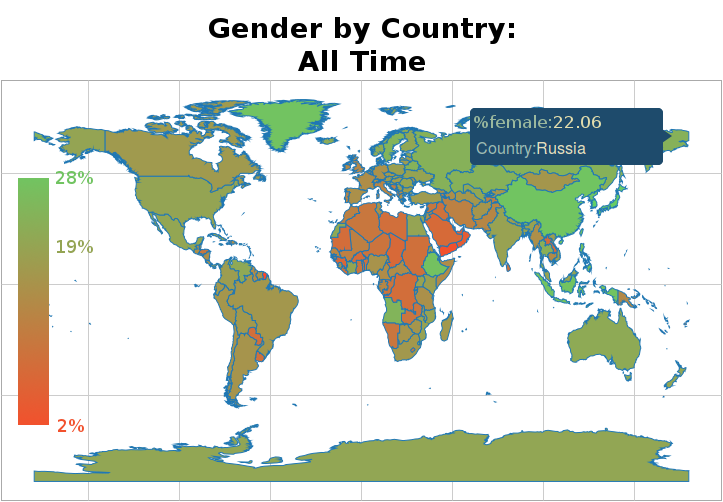
\includegraphics[width=\columnwidth]{figures/genderbycountry.png} 
\caption{The Wikidata female ratio of biographies aggregated by place of birth and citizenship. The greener colours indicate a higher ratio of humans that are born-in or are citizens-of that country are women. For instance China, Korea and Japan each approach 28\%, whereas Russia is about 22\%, the United States 19\%, and the lowest is Yemen at 2\%. This data is represents the January 3\textsuperscript{rd} 2016 snapshot.}
\label{fig:genderbycountry}
\end{figure}


\subsection{Snapshots}
All of our data is derived from the official Wikidata database downloads, which represent a cross-sectional ``snapshot'' of Wikidata as it was at a specific date. Wikidata releases new snapshots weekly. We re-process each of the 11 indicators for every new snapshot, and additionally compute the differences that occurred between the newest snapshot and the second-newest. This allows us to monitor activity on Wikidata at a weekly level of granularity. For instance Figure  \ref{fig:genderbydob} and Figure \ref{fig:genderbycountry} show the state of the date of birth and country indicators, \textit{for all time}, as of the January 3\textsuperscript{rd} 2016 snapshot, but Figure \ref{fig:genderbylang} shows the \textit{changes} of the week between December 27\textsuperscript{th} 2015 - January 3\textsuperscript{rd} 2016.

Therefore, we are also generating a dataset of \textit{weekly changes} which allows us to \textit{monitor} the status of biographies in Wikidata. We can inspect the changes in composition of genders, or date of birth, which can speak to efforts from Wikipedian communities attempting to counter bias in the database. 


\subsection{Technical Details}

Note that for fidelity there is virtually no data-cleaning done, as the point of our project is to display information as faithfully as possible. Our dataset is meant to be used to uncover potential biases in Wikidata and the world at large, so we feel that any cleaning process would introduce further biases. An instructive illustration of this is that the ``gender'' property in Wikidata is actually labelled in English  as ``sex or gender'' (no distinction), and not limited to any value. Over our time snapshotting we found 36 values used for ``sex or gender'', including ``male'' and ``female'', but extending to non-binary genders ``transgender female'', ``intersex'', ``fa'afafine'', ``transgender'', ``Gender fluid'',  ``genderqueer'', ``kathoey'', and ``queer''. At times the other categories of information are recorded here - perhaps erroneously - such as ``gay'', or ``homosexuality''. Cleaning this data would be a disservice, we feel, to communicating how Wikidata is used.


Code used to generate these indicators are available online, freely licensed. Our first snapshot is from September 17\textsuperscript{th} 2014, and tracks the official  Wikidata data dumps, updating weekly. We archived the January 3\textsuperscript{rd} 2016 version as a quality-checked, canonical version \footnote{\url{WEBSITE BLINDED}}. All our code to make this data and the analyses presented here using both \textit{python-pandas} and \textit{R} can be found in our github repository \footnote{\url{WEBSITE BLINDED}}.

Note that the missing data in the first half of 2015 is the period in which automatic collection these statistics was under construction.

\begin{figure}
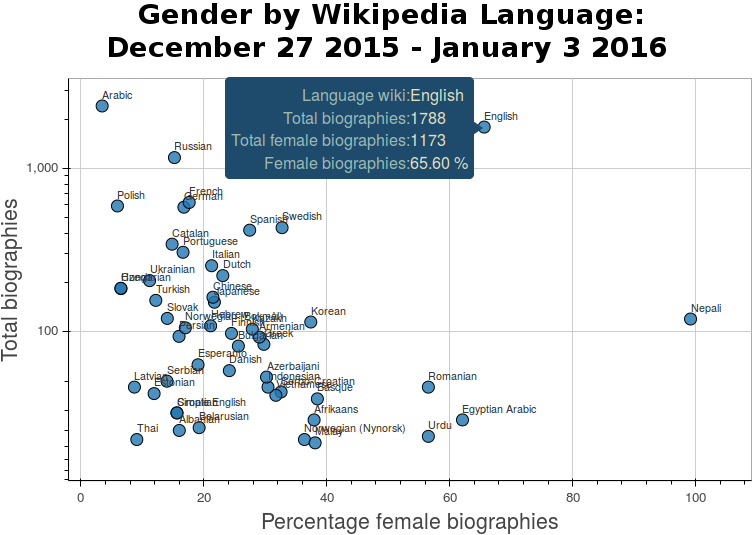
\includegraphics[width=\columnwidth]{figures/genderbylang.png} 
\caption{The changes in the size and percentage of female biographies for large Wikipedia languages in the period December 27\textsuperscript{th} 2015 - January 3\textsuperscript{rd} 2016. English Wikipedia Increased 1,788 biographies 65\% of which were about women. Meanwhile Nepali Wikipedia increased by 120 biographies, 119 of which were about women.}
\label{fig:genderbylang}
\end{figure}


\section{Results}
\subsection{RQ1: Real world validation of WHGI}
This project is not the first to establish that Wikipedia data has real-world biases via correlation to exogenous indicators. In 2008 Rask concluded that Wikipedia editions displayed real-world \textit{socio-economic} disparities similar to those found in the United Nations Human Development Index (HDI) \cite{rask_reach_2008}. Rask identified three limitations with their study (1) they used only 11 Wikipedia languages (2) they suggested longitudinal analysis be carried out, and (3) language-disaggregation is only a proxy for country-disaggregation which the HDI utilizes. WHGI overcomes all three of these limitations as it measures all 285 Wikipedia languages, updates weekly, and handles by-country-disaggregation. Although we are not focused on \textit{socio-economic} disparities but \textit{gender} disparities we still investigate exactly how well WHGI reflects the real world, and validated our indicators by comparing it against 3 exogenous datasets. We correlated the WHGI by date of birth versus historical world population trends; WHGI by country versus global gender-disparity indices; and WHGI by occupation versus United States Bureau of Labor Statistics occupation gender.

\subsubsection{World Population} Our first validation is a ``sanity check'' to compare the world's population by year to the number of humans in WHGI by year of birth. We conduct this validation even though the number of people alive and the number of Wikipedia-notable people born are different measures. However if we operate under the assumptions that (a) the proportion of the world population which is Wikipedia-notable is constant over time and (b) that the birth rate is a fixed proportion of the population, then theoretically their curves should share approximately the same shape.

We performed a standard Pearson correlation between the number of people in Wikidata born in a particular year, and the estimated historical world population by the US Census
Bureau\footnote{\url{https://commons.Wikipedia.org/wiki/File:Population_curve.svg}}. The Census Bureau has estimates of world population from 10,000 b.c.e. to 2001, and Wikidata from 4203 b.c.e. to 2015. We conducted this correlation for our earliest and latest snapshots - the population statistics of Wikidata at September 17\textsuperscript{th} 2014, and again separately at January 3\textsuperscript{rd} 2016. The results in Table \ref{table:worldpop} show a high and significant correlation between real world estimates and Wikidata, almost constant at 0.85. Overall though the population of Wikidata over time seems very aligned with the World's population over time, so Wikidata at least is a ``sane'' representation of the world.

\begin{table}
\caption{Correlation of number of WHGI by date of birth and world population. Significances are $ ^{**}p\leq 0.01$.}
\label{table:worldpop}
\begin{tabular}{lrrrr}
\toprule
snapshot &  Pearson correlation \\
\midrule
2014-09-17 & 0.852**  \\
2016-01-03 & 0.845**  \\
\bottomrule
\end{tabular}
\end{table}

\subsubsection{Exogenous Gender-Disparities Indices}

WHGI is inspired, in part, by the rich landscape of gender disparity indices. This type of index ranks countries by a measure of gender equality. If we aggregate WHGI by place of birth and citizenship, and look at the female ratio of humans, we too have a country-by-gender equality measure\footnote{Despite having the same by-country unit of analysis with this aggregation WHGI is not an ``index'' like those we compare it to, since an index weights and combines many indicators \cite{rossi_handbook_1980}. }.  We correlated the country rankings of this WHGI aggregation with 4 popular exogenous indices to see how well Wikidata reflects real world gender disparities.

The 4 exogenous indices we used were: The traditional United Nations' Gender Development Index (\textbf{GDI})  \footnote{\url{http://hdr.undp.org/en/content/gender-development-index-gdi}} which considers disparity in income, education, and life expectancy. Social Watch's Gender Equity Index (\textbf{GEI}) \footnote{\url{http://www.socialwatch.org/node/14366}} tries to broaden the scope of the variables by not only incorporating education and economic participation, but also stretching into economic and political empowerment. The Global Gender Gap Index (\textbf{GGGI}) \footnote{\url{http://reports.weforum.org/global-gender-gap-report-2014/}} grows yet wider by covering all previous topics and along more detailed dimensions. And most recently  the Social Institutions and Gender Index (\textbf{SIGI}) \footnote{\url{http://www.genderindex.org/ranking}} has attempted to capture disparity in norms, values and attitudes.

For each index we conducted a calibration step, to find the date of birth start and end inclusion years which maximized our correlations. In each case the maximizing start year was found to be between 1900 and 1910 and the end year to be 2015. We interpreted the found thresholds as a good sign firstly because the exogenous indices are measures of recent history too, and secondly because it shows a robustness in the way that WHGI relates to exogenous indices.

We repeated the index correlations twice, once using the September 17\textsuperscript{th} 2014 snapshot of Wikidata, and then using January 2016 data. That is, we have correlations between rankings of countries given by exogenous indices and Wikidata - at two separate times.

Table \ref{table:scores} shows the correlations with each index, all of which were significant and ranged from 0.278 to 0.457. Affirmingly, when looking at this information through a longitudinal lens, the correlation with every index is increasing over time at which we sampled Wikidata. On the low end the GDI correlation grew by 7.6\%, and on the upper end, the SIGI correlation jumped 24.5\% in the about-a-year time frame between Wikidata snapshots. Because we are using the  female ratio of biographies by country and not the absolute number of biographies these correlation are not growing simply because of increased number of data points.

\begin{table}
\caption{WHGI-country correlation to external indices. Correlation is the Spearman $\rho$, and significances are $ ^*p\leq 0.05 $, $ ^{**}p\leq 0.01$.}
\label{table:scores}
\begin{tabular}{lrrrr}
\toprule
snapshot &  GEI &  SIGI &  GGGI &  GDI  \\
\midrule
2014-09-17 &  0.417** &       0.338** &          0.310* &         0.278**  \\
2016-01-03 &  0.457** &       0.402** &          0.386** &         0.299**  \\
\bottomrule
\end{tabular}
\end{table}

Previous analyses showed that WHGI being most closely correlated with  GEI, and least to GDI has implications for Wikipedia's notability policy. Where they both measure gender gap in school enrolment, years of schooling, and earned income, GEI additionally measures positions of power, and GDI life expectancy. That means that notability in Wikipedia is more correlated to power in society than it is to health status \cite{BLINDED}. This analysis is remains true in 2016, as the order of the strengths of the correlations has remain unchanged. Still the the strengths of those correlations has increased across all indices, which means that the gender disparities found in WHGI by country are increasingly looking \textit{more} like these real world gender disparities.


\subsubsection{Occupation Gender}
The notion of what a human's job or occupation is, we saw in Table \ref{table:accompanying}, is well recorded in Wikidata. To answer the question of how representative of the real world Wikidata's gender by occupation is, we compared it to data from the United States Bureau of Labor Statistics (BLS) \footnote{\url{http://www.bls.gov/cps/aa2012/cpsaat11.htm}}. We borrow this ground truth technique from \cite{kay_unequal_2015} who used it to evaluate the gender representation of Google image search results for occupation key terms.

Approximately 60\% of our sample have occupation data, and together over 4,000 occupations are represented. The BLS has 332 occupation categories which are at a higher level ontologically than  recorded in Wikidata. Whereas Wikidata might record that someone is a pastry chef, the BLS only has a category for cooks. In order to match the indicators we used Wikidata's internal ontology hierarchy to generalize the occupation terms. A \textit{subclass of} property exists in Wikidata, that relates items to their more general concept - which we can use for occupations. Wikidata describes that pastry chef is a \textit{subclass of} chef, and that chef is a \textit{subclass} of cook. 

Our method was to raise the generality of Wikidata occupations until there were less than 500 occupations to ease the matching task. Two authors then matched occupations manually for accuracy and confirmation. We resolved disagreements until the sets were matched. However not all occupations could be matched due to the specificity of the BLS, rendering coverage of Wikidata occupations 57\% complete. The largest occupations in Wikidata were sportsperson and politician, and neither of them had matches in the BLS. In the reverse, there were many BLS occupations for which Wikidata did not have any matching occupations, such as ``lodgings manager''. This outlines a limitation of this validation, that being a lodgings manager does not inherently make you notable for inclusion in Wikipedia. 

It must be acknowledged that the BLS data describes the United States whereas WHGI has a worldwide scope. However with WHGI restricted only to biographies with place of birth in the United States the correlation becomes only marginally siginificant. This might be due to the fact that the population in Wikidata that has both occupation and place of birth recorded are particularly notable people, and contain even less of the everyday occupations that the BLS does.

Finally we correlated the rankings of the list of most gendered occupations according to WHGI to that of the BLS. We did this for early and late snapshots, but because occupation was not a property that we initially recorded, our first snapshot which included occupation was August 9\textsuperscript{th} 2015.  Table \ref{table:bls} shows the spearman rank correlation found was a significant 0.410, and since then the correlation has increased to 0.473. These are moderate correlations which we claim support a link that Wikidata reflects the real world, and like the by-country indicator is becoming increasingly more accurate.

\begin{table}
\caption{Rank correlation of gender ratios by occupation between WHGI and US
Bureau of Labor Statistics. Signficances are $ ^{**}p\leq 0.01$.}
\begin{tabular}{lrrrr}
\toprule
snapshot &  Spearman Rank Correlation \\
\midrule
2015-08-09 & 0.410**  \\
2016-01-03 & 0.473**  \\
\bottomrule
\end{tabular}
\label{table:bls}
\end{table}


\subsection{RQ2: Impact on Wikipedia Communities}
Another main purpose for investigating this dataset is to support and provide metrics for Wikipedians communities attempting to  address content gaps. Therefore we turn to focus on statistics of our dataset with regard to how it has changed over time as these Wiki\-pedian communities have been edting. 

\begin{figure}
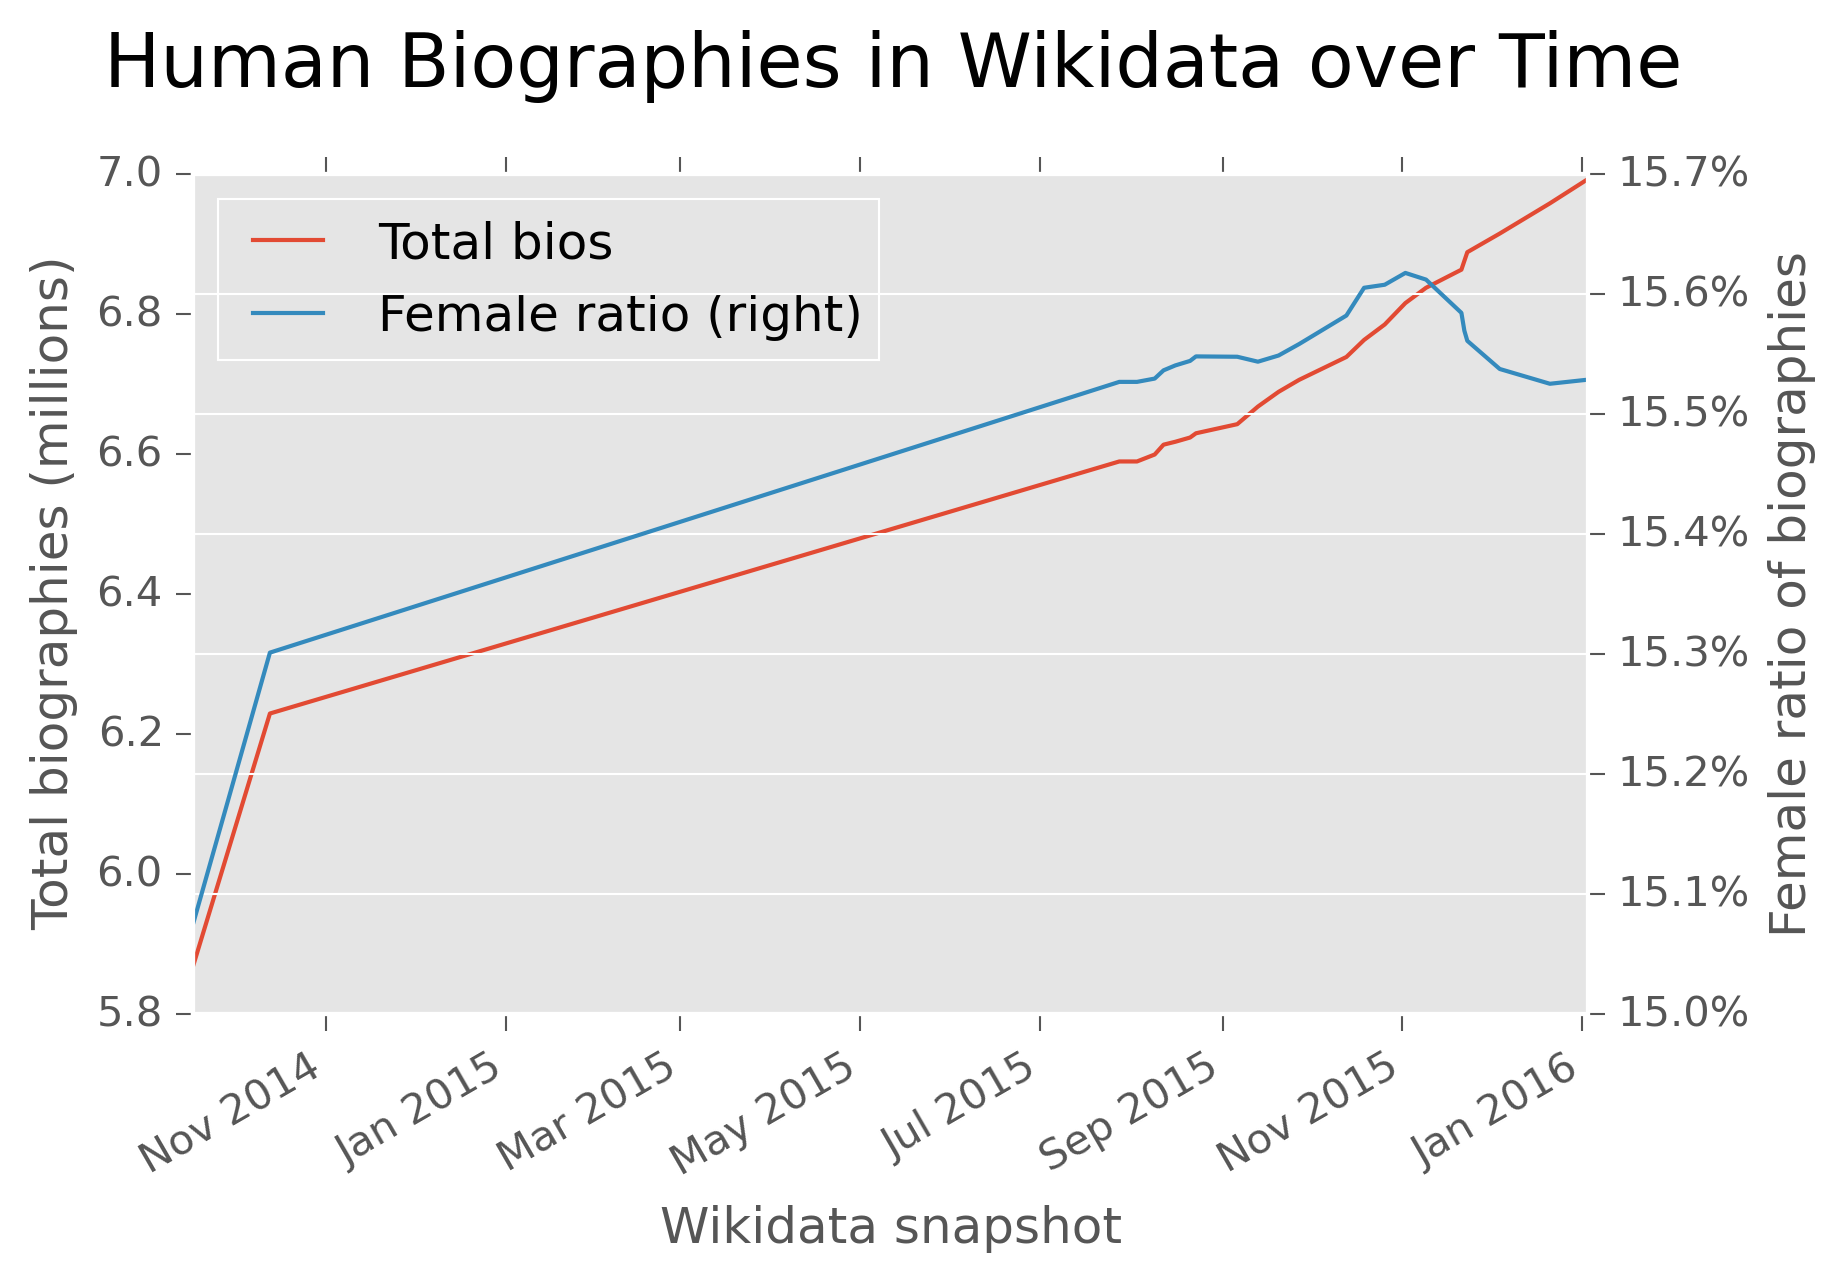
\includegraphics[width=\columnwidth]{figures/totalfrb.png} 
\caption{Total number of human biographies (left) and the female ratio of those biographies (right) by Wikidata snapshot. The total number of humans found in Wikidata over time is displaying linear, unconstrained growth. Over the same time the female ratio of biographies in Wikidata has risen by 0.5\%.}
\label{fig:totalfrb}
\end{figure}

First we queried the way the total number of biographies and the ratio of women represented as Wikidata has evolved. Total humans in Wikidata increased from 5,869,606 to 6,999,542, and shows linear, unconstrained growth (see Figure \ref{fig:totalfrb}). Certainly Wikidata is active and changing, but how? An important measure for content-focused communities is the ratio of biographies which are about women, as espoused in \textit{WikiProject Women in Red}\footnote{\url{https://en.wikipedia.org/wiki/Wikipedia:WikiProject_Women_in_Red}}. We looked into the ratio of  humans recorded ``female'' versus all gendered biographies. Similar to total biographies this measure is rising at a fairly linear rate of approximately 0.5\% per year (Figure \ref{fig:totalfrb}). The final months on record show a slight decline which warrants further investigation. 

\begin{figure}
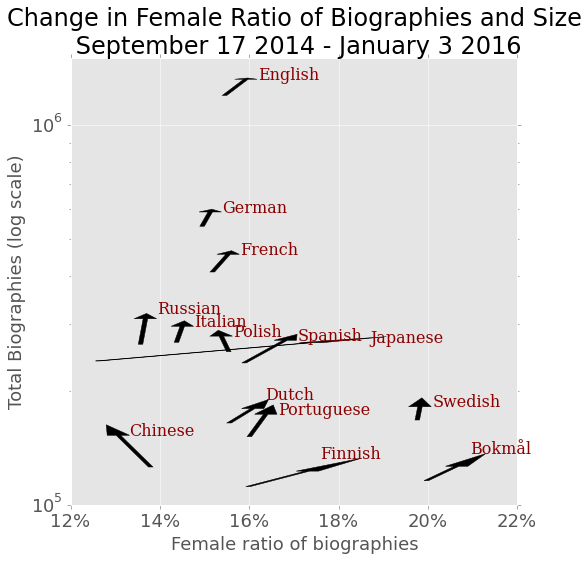
\includegraphics[width=\columnwidth]{figures/arrowplot_flippedaxes.png} 
\caption{The change in female ratio of biographies and total biographies over time, of Wikipedia languages with 100,000 or more gendered biographies. The tail of the arrow represents the Wikipedia's position in September 2014, and the head in January 2016.}
\label{fig:changefrb}
\end{figure}

We took a more granular look at the evolution of the female ratio of biographies by disaggregating by Wikipedia Language in Figure \ref{fig:changefrb}. Of the languages that have 100,000 or more gendered biographies, and during the time period September 17 2014 to January 3 2016 all Wikis increased in size of total biographies. In terms of the rate of women represented in biographies, Norwegian (Bokm\aa l), Spanish, English, Finnish, and Dutch Wikipedias each increased by more than 0.5\% points. Japanese however jumped the most, by 4\% points, more than any other language. 

Japanese Wikipedians relate this increase to strong editing activity about women who are idols, models and celebrities, despite an effort to delete biographies about Adult Video idols\footnote{\url{BLINDED}}. We hypothesize this deletion effort may also be partially responsible for the decline viewable Chinese Wikipedia and the decline in total ratio seen in Figure \ref{fig:totalfrb}.

Are these changes in the Wikipedias correlated with the efforts of Wikipedian communities targeting gendered content?

There are many Wikipedian communities who's goal it is is to increase the coverage of Women's biographies, for instance: Wiki\-Project Women Scientists \footnote{\url{https://en.wikipedia.org/wiki/Wikipedia:WikiProject_Women_scientists}}, Art + Feminism\footnote{\url{http://art.plusfeminism.org/about/}}, and Women in Red, just to name a few. One concern of these organizations is if their editing efforts are making large scale impacts on the Wikipedia. Fortunately Wikiproject Women in Red keeps metrics of how many biographies they add on a monthly basis, and we were able to conduct a cross-correlation between the time-series of monthly number of biographies created by Women in Red, and the number of female biographies added to English Wikipedia. The correlation between these activities is 0.657, which indicates a positive link. Even if we cannot determine a causal relationship between editing efforts and the increase in women's representation in these languages we are still able to numerically highlight this trend which was not viewable before.

\begin{figure}
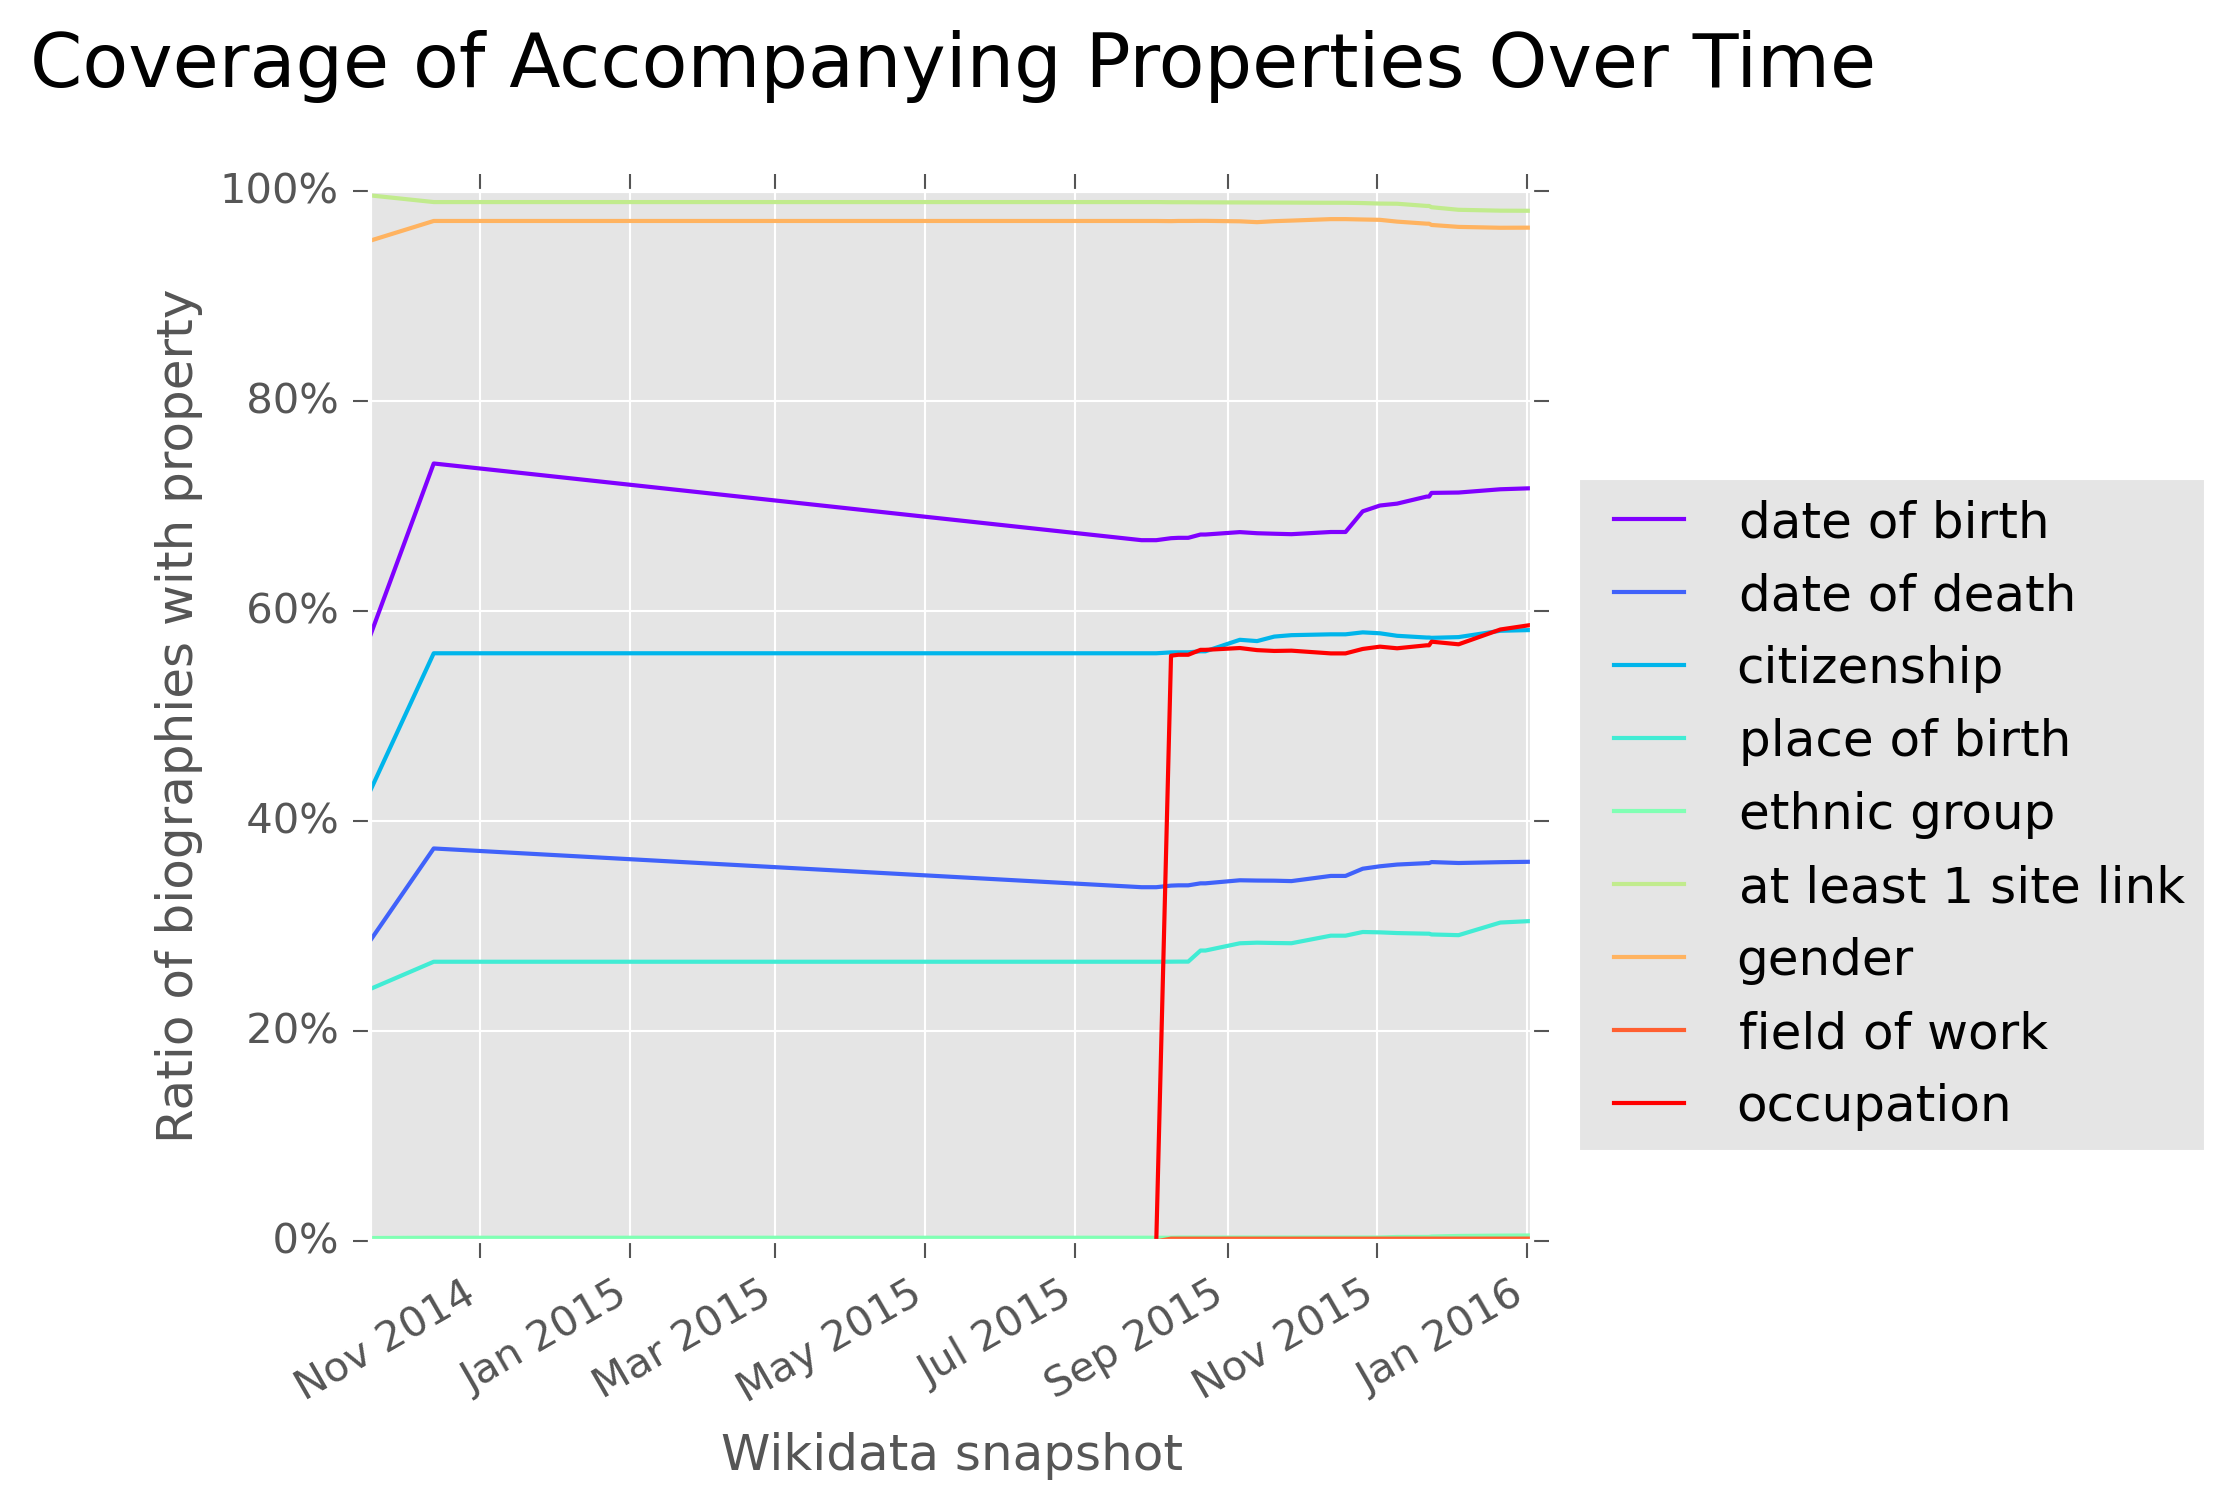
\includegraphics[width=\columnwidth]{figures/additionalprops.png} 
\caption{Trends of property coverage by Wikidata snapshot. Most humans have at least one Wikipedia article (``site link'') and a recorded gender, other properties are slowly increasing in coverage.}
\label{fig:accompanying}
\end{figure}



\subsubsection{Data Quality}
Of course the female ratio of biographies is not the only way to characterize the effect of content-focused editing, we might also inquire to the wider quality of biographies in Wikidata. One way to investigate data quality is the coverage of demographic  properties on these biographies. Figure \ref{fig:accompanying} and Table \ref{table:accompanying} show the trend in coverage of all properties at the earliest and latest WHGI snapshots and the latest DBpedia snapshot\footnote{\url{http://wiki.dbpedia.org/services-resources/datasets/dataset-2015-10/dataset-2015-10-statistics}}. The statistics show that data quality has been increasing across all properties over time. The number of humans with \textit{gender} data increased just 1\% point but is close to complete at 96\% coverage, DBpedia does not clearly display gender completeness data. In the time domain however \textit{date of birth} and \textit{date of death} coverage increased by 14\% points and 7\% points respectively. This means that date of birth and death cover about $\frac{3}{4}$ and $\frac{2}{3}$, of the biographies, both counts of which exceed DBpedia which count less than $\frac{1}{2}$ and $\frac{1}{4}$ respectively. \textit{Place of birth} jumped by 6\% points to $\frac{1}{3}$ coverage, however this lags behind DBpedia's strength in this domain at $\frac{4}{5}$.

In terms of Wikidata specific property coverage \textit{Citizenship} data increased the most, by 15\% points and is available for more than half of humans, Next \textit{ethnic group} doubled, but just to 0.6\% coverage. Lastly, \textit{field of work}, and \textit{occupation} data was not included in our dataset until later, so their growth, while increasing, is not precisely comparable.


Curiously, the rate of humans having at least one Wikipedia article decreased slightly, and this has an important interpretation. A Wikidata human without a Wikipedia article is known as a ``structural item'', for instance a member of royalty without a Wikipedia article but is needed to make a family tree complete. With the view that a structural item is an artefact from editors paying attention to Wikidata's structure, the decrease in the ratio of sitelinked humans can also be seen as an increase in data quality. 

\begin{table}
\caption{Change in rates of property coverage for humans between earliest and latest snapshots and DBpedia 2015-10}
\begin{tabular}{lrrr}
\toprule
{} &  2014-09-17 &  2016-01-03 & DBpedia 2015-10\\
\midrule
gender               &       95.3\% &       96.5\% & n/a \\
date of birth        &       57.6\% &       71.7\% & 45.3\% \\
date of death        &       28.6\% &       36.1\% & 17.8\% \\
citizenship          &       42.8\% &       58.2\% & n/a \\
place of birth       &       24.0\% &       30.5\% & 80.0\% \\
ethnic group         &        0.3\% &        0.6\% & n/a \\
field of work        &        n/a &        0.3\% & n/a \\
occupation           &        n/a &       58.7\% & n/a \\
at least 1 site link &       99.6\% &       98.1\% & n/a \\
\bottomrule
\end{tabular}
\label{table:accompanying}
\end{table}

\subsection{RQ3: Impact on Research}

\begin{table}
\caption{The relative risk for biography article quality to be misaligned with readership demand (in English Wikipedia). Here we see that biographies about women are 30\% more likely to have readership outstrip article quality (Needs Improvement), conversely biographies about men are 14\% less likely to need improvement. Spent Effort are the cases where article quality exceeds readership demand.}
\begin{tabular}{lrrr}
\toprule
{} &  Needs Improvement &  Spent Effort \\
\midrule
Female        &               1.30 &          1.03 \\
Male          &               0.86 &          1.15 \\
Non-binary    &               2.65 &          0.50 \\
Non-biography &               1.03 &          0.95 \\
\bottomrule
\end{tabular}
\label{table:pah}
\end{table}

As well as providing metrics for Wikipedian communities to monitor and potentially address the content gap, WHGI can also be used in collaboration with other quality measures to impact research, particularly to enhance our understanding of the gender disparity phenomenon in Wikipedia and shed light on the underlying mechanisms in peer production communities.

 For instance Warncke-Wang et al. explored supply and demand misalignment in Wikipedia by looking at the difference in actual and predicted article quality using page-views \cite{warncke-wang_misalignment_2015}. They cite examples of over-demanded articles where readership exceeds quality (e.g. ``Wedding'', and ``cisgender'') and over-supplied articles where quality exceeds readership (e.g. ``Themes in Robert Browning's poetry''). Following these examples, they follow up with a broader investigation of patterns in misalignment by using WikiProjects to categorize articles. For example, they find that the reader demand of WikiProject:LGBT (Lesbian, Gay, Bisexual, Trans*) far exceeds Wikipedia's supply: articles in Wikiproject LGBT are 9 times more likely to be found in the ``Needs Improvement'' dataset compared to the project's overall representation in Wikipedia. They dub this the \textit{relative risk}\cite{davies_when_1998}.

We can further our understanding of the extent and nature of gender disparity in Wikipedia by combining our WHGI metrics and Warncke-Wang's supply-demand misalignment approach. We started with the exact same dataset in Warncke-Wang et al's paper and re-ran this analysis. Instead of aggregating by WikiProject, we utilized the WHGI and were able to aggregate by gender over the entire encyclopedia. Table \ref{table:pah} shows the relative risk for gendered biographies being either in need of improvement (over-demanded), or showing extra ``spent effort'' (over-supplied). Our findings show that women's biographies are 30\% more likely to be in the category of ``needs improvement'', where as men's biographies are 14\% less likely. Women's biographies are roughly comparable to the average encyclopedia article in terms of belonging to the ``spent effort'' category, whereas men's biographies show a 15\% higher likelihood.

The row ``non-binary'' speaks to the approximately 50 biographies whose gender is neither ``male'' nor ``female'', and shows twice the likelihood to need improvement, $\frac{1}{2}$ the likelihood to represent spent effort. As a control, we also calculated the relative risk of every article which is not a biography, in the ``non-biography'' row, which sensibly shows a close-to-baseline result in all categories. 

Another example of how WHGI could be useful for researchers is that the time series nature of the WHGI dataset enables an alternative outcome metric to measure the efficiency of a range of content improvement movements and strategies in Wikipedia. Researchers have long been interested in understanding the effectiveness of content-improvement movements, ranging from formally organized efforts such as APS Wikipedia initiatives \cite{farzan_wikipedia_2013} and Wikipedia Education Program \cite{warncke-wang_success_2015}, to members self-organizing activities such as Collaboration of the Week, WikiCup, Today's article for Improvement \cite{zhu_organizing_2012}\cite{warncke-wang_success_2015}. To measure the success of these movements, the prior research has been using outcome metrics such as number of revisions \cite{zhu_organizing_2012}\cite{farzan_wikipedia_2013}, and Wikipedia's article quality measurement and machine predicted quality measurement \cite{warncke-wang_success_2015}. WHGI can provide a new success metric - the gender ratio of the biographic articles created by a particular movement - to provide a new angle to examine the efficiency of these movements in improving the content coverage in Wikipedia.

Overall, the above two examples illustrate how WHGI could be useful for researchers, in potentially improving our understanding of the gender disparity phenomenon and the effectiveness of different content improvement movements in Wikipedia.

   
\section{Discussion}
We established the WHGI, and using longitudinal analysis showed that women are increasingly being represented in most Wikipedias. This, along with the fact that exogenous validations show that Wiki\-pedias' gender disparities are increasingly reflecting the real world suggest that Wikipedia is ``catching up'' to real world disparities. Further, this catching-up is also correlated to the activity levels of women-focused editing initiatives.

We also saw that even as all Wikipedias are growing in total biographies and data coverage, their inclusion of women differs. This leads very naturally into asking about the gendered implications of notability policies, and could be tested using WHGI and propensity score matching. That is, for a language which has a implemented a stricter notability policy we could compare the way that language's gender compostion changes against a language which was on a similar trajectory before the change, but retained its notability policy.

Moreover WHGI we demonstrated that WHGI is generally useful to match with other datasets and provide large-scale gender insights. With the supply-demand misalignment dataset we were quickly able to show that women's biographies are 30\% more likely to be over-read compared to their article quality. This analysis serves as an example of how more data connections could be made. 

Beyond the Wikipedia-research landscape, a historian could use the data to determine the gender-disparity levels of a specific place and time. Typically to quantify the gender climate one would rely on the indices like those mentioned in the exogenous indices section. However these indices, are limited to discussing recent history. Our validation showed that our data is in touch with the real world. With this dataset we can quantify a type of gender-disparity of medieval France, ancient Greece, or Ming dynasty China. WHGI is useful in all the same ways that exogenous indices are used, only with a larger timespan. That is an approach not possible before Wikidata.

\section{Limitations and Future Work}
WHGI is a proxy for real world phenomena, but is also limited by the worldview of Wikipedia editors and is constrained by its notability policies. 
Wikipedia's notability policies require humans to be in positions of power which are systemically biased against women, how then can the general rise in women's biographical representation be explained? There could be several possible reasons. At least three factors that affect encyclopedic inclusion are: (1) the rate at which women receive positions of power in the real world, (2) the level of gender bias in Wikipedias' notability policies, and (3) the level of efforts to write about women in Wikipedia. 

The validation analysis (correlations with existing gender disparity indices) show that WHGI captures real world phenomena. Since we were able to look at the fine-grained intra-year level, the increased correlation with existing gender disparity indices between our earliest and latest snapshots indicates that WHGI is capturing movement in the latter two factors - policy changes and editing effort changes in the Wikipedia community. Unfortunately we cannot disentangle the influence in these three factors.

Yet another limitation is that there may also be biography articles in Wikipedias that are not recorded as humans in Wikidata. However the size of this set is not readily computable our best estimates come from the latest DBpedia extract which contains 3,158,512 humans - 122,276 or 4\% more than Wikidata. Particularly we would like to know how much growth in Wikidata stems from Wikipedia's growth (e.g. a new biography is added), or migration of information to Wikidata (e.g. an existing biography in Wikipedia is marked as a human in Wikidata).

Still applications on top of WHGI indicators could be built to help the community, for instance to detect spikes in creation and deletion of specific demographics of humans. Such a tool could also alert to the presence of unplanned activity, good or bad, which affects the macro-level gender of Wikipedia and Wikidata. Take Figure \ref{fig:genderbylang}, it shows a week where contributions to Nepali Wikipedia are nearly 100\% about women. Likewise, if a week were to show a net-subtraction of female biographies a community alert could be generated.

We wonder if tools like this would be motivating as well, as well as simply measuring progress. This would suggest a path of research investigating how editors use information to act. As it happens Women in Red already cite WHGI for data, but would a tighter integration help the cause? A user study in providing editing communities with detailed feedback and exact movement in the landscape would ask if ``what gets measured, get fixed'' - more quickly?
 

\section{Conclusion}
We made the Wikidata Human Gender Indicators (WHGI), a biographic database for researchers wishing to incorporate gender data along dimensions of time, space and occupation. Based off of Wikidata and Wikipedia it can most obviously be used by those communities to monitor the effects of focused editing and biases in their content. We also validated the indicators with measures of the real world, such as population, country-based gender disparities, and occupations. These validations showed that the WHGI is significantly correlated to real world demographics and gender disparities. We also showed that data quality of Wikidata has been increasing. Data quality and correlations increasing together is particularly encouraging as support for using WHGI as a tool, as we showed extending previous research in article-readership misalignment. WHGI is freely available for download, we have outlined some of the potential ways in which it could be used, and hope that many more are thought of by others.


\section{Acknowledgments}
We acknowledge the hard work done by Wikimedians in countering systemic bias. We hope to continue running the open source project in service of the Wikipedia and research communities seeking to statistically describe gender disparities. The ways in which we expand WHGI we hope will be directed by user's feedback.

We are especially grateful to the Wikimedia Foundation for funding us through an Individual Engagement Grant. 

We are also especially grateful to the Wikidata and Wikidata Toolkit teams.



%
% The following two commands are all you need in the
% initial runs of your .tex file to
% produce the bibliography for the citations in your paper.
\bibliographystyle{abbrv}
\bibliography{wigi-dataset-opensym}  % sigproc.bib 
\end{document}
